\documentclass[11pt,a4paper]{article}
\usepackage[T1]{fontenc}
\usepackage[utf8]{inputenc}
\usepackage[english]{babel}
\usepackage{lmodern}
\usepackage{microtype}
\usepackage[margin=2.3cm]{geometry}
\usepackage{graphicx}
\usepackage{booktabs}
\usepackage{float}
\usepackage{caption}
\usepackage{csquotes}
\usepackage[style=numeric-comp,sorting=none,backend=biber,maxbibnames=4]{biblatex}
\usepackage[hidelinks]{hyperref}
\usepackage[capitalise]{cleveref}
\addbibresource{references.bib}
\graphicspath{{../../results/figures/}}
\captionsetup{font=small,labelfont=bf}

\title{L band (NISAR) versus C band (Sentinel-1)\\for detecting a clear-cut in the Vosges mountains\\[0.4em]
\large Feasibility test preparing the SERTIT / ICube internship}
\author{Mamadou Galy Diallo}
\date{November 2026}

\begin{document}
\maketitle

\begin{abstract}
\noindent
This test compares how well NISAR (L band, 24~cm) and Sentinel-1 (C band, 5.6~cm) distinguish a recent clear-cut
from the neighbouring intact forest.
\begin{itemize}
\item \textbf{Site}: a 2.36~ha clear-cut made in early August 2026 in the Vosges mountains, dated and delineated
  with Sentinel-2.
\item \textbf{Data}: NISAR level-2 products generated by ISCE3 (GUNW coherence, GCOV HH/HV backscatter) in three
  geometries, and a series of 13 Sentinel-1 images processed with SNAP, all brought onto a common 20~m grid.
\item \textbf{Metrics}: separability is measured with the AUC, Cohen's d and the Jeffries-Matusita distance, with
  block-bootstrap confidence intervals.
\end{itemize}
Results:
\begin{itemize}
\item \textbf{Coherence}: at L band, the pair spanning the cut separates cut and forest almost perfectly
  (AUC 0.995; coherence 0.29 vs 0.69), even over 24~days. At C band the forest is already decorrelated after
  12~days (0.28), and coherence adds almost nothing (AUC 0.71--0.74).
\item \textbf{Backscatter}: in ascending geometry, the cross-polarisation drop reaches $-4.3$~dB at L band
  (AUC 0.97), against $-2.2$~dB at C band (AUC 0.91). At equal (descending) geometry, however, C band performs as
  well as L band (AUC 0.91 vs 0.84).
\item \textbf{Persistence}: in ascending geometry, the L-band contrast persists until November, whereas the C-band
  contrast weakens in October; in descending geometry, persistence is similar in both bands.
\end{itemize}
Hypotheses H1, H2 and H4 are confirmed on this site; H3 is only partly confirmed. The robust advantage of L band is
interferometric: for backscatter, it depends on the acquisition geometry. The processing chain, written as reusable
Python modules, can be transferred directly to the future Copernicus L-band mission ROSE-L.
\end{abstract}

\tableofcontents
\newpage

%=====================================================================
\section{Context and objective}

The SERTIT / ICube internship explores L and P bands (NISAR, BIOMASS) for the detection of deforestation and
landslides.
\begin{itemize}
\item \textbf{NISAR}: since 2025, the NASA-ISRO NISAR mission~\cite{kellogg2020nisar,nisar2018handbook} provides,
  for the first time, systematic, free and open L-band data over Europe. Its level-2 products are generated by
  the ISCE3 software~\cite{isce3} and distributed by ASF~\cite{asf2026nisar}.
\item \textbf{ROSE-L}: in Europe, L band will then be provided by the Copernicus ROSE-L mission, with launch planned
  for 2028~\cite{esa2020rosel}.
\item \textbf{BIOMASS}: P band (BIOMASS~\cite{quegan2019biomass}) does not acquire over Western Europe (SOTR
  exclusion zone) and remains a perspective.
\end{itemize}

Operational radar detection of forest cuts and disturbances currently relies on Sentinel-1
C band~\cite{torres2012sentinel1}. It uses the backscatter decrease and the shadowing effect at the cut
edge~\cite{bouvet2018shadow,reiche2021radd}. L band has proved more sensitive to forest
structure~\cite{joshi2015mapping}. The aim of this test is to check, on a real case and with the new NISAR
products, whether L band brings a measurable gain over C band for separating a recent clear-cut from intact forest.

\subsection{Question and hypotheses}

\emph{On a recent clear-cut in the Vosges (June--November 2026), do NISAR (L band) interferometric coherence and
backscatter separate the cut from intact forest better than Sentinel-1 (C band)?}

\begin{description}
\item[H1] In intact forest, 12-day coherence is higher at L band than at C band. L band scatters on trunks and large
  branches, which are stable, whereas C band is dominated by moving foliage.
\item[H2] The coherence difference between cut and forest is therefore larger at L band.
\item[H3] The backscatter decrease after the cut is stronger at L band, since C band saturates over dense forest.
\item[H4] Cross-polarisation (HV) is the most sensitive backscatter indicator, being linked to volume scattering
  and hence to biomass.
\end{description}

%=====================================================================
\section{Data}

The inventory of the ASF catalogue (\texttt{asf\_search}~\cite{asfsearch}) covered the Vosges / Alsace footprint
from June to November 2026. It listed 546 NISAR products, including 93 GCOV and 67 GUNW, and 263 Sentinel-1 IW SLC
images over five relative orbits. The data used are summarised in \cref{tab-data}.

\begin{table}[htbp]
\centering\small
\caption{Data used on the site.}
\label{tab-data}
\begin{tabular}{p{2.6cm}p{5.6cm}p{6.6cm}}
\toprule
Sensor & Products & Details \\
\midrule
NISAR (L, 1.26~GHz) & L2 GCOV ($\gamma^0$ HH, HV, RTC) and GUNW (HH coherence), produced by ISCE3,
\emph{provisional} status & 3 geometries: A144~F26 and A72~F26 (ascending), D138~F64 (descending). 10 to 11 GCOV and
8 to 9 GUNW per geometry, from 19/06 to 10/11/2026. 12-day pairs; the pair spanning the cut is 24 days long (an
acquisition is missing at the end of July). \\
Sentinel-1 (C, 5.4~GHz) & IW SLC, VV+VH & Descending orbit 139, sub-swath IW2. 13 dates 12 days apart, from 14/06
to 06/11/2026 (S1A then S1C). \\
Sentinel-2~\cite{drusch2012sentinel2} & L2A, NDVI & Reference: delineation and dating of the cut (30 clear
dates). \\
ESA WorldCover~\cite{zanaga2022worldcover} & 2021 map, 10~m & Forest mask. \\
\bottomrule
\end{tabular}
\end{table}

Downloading everything would have taken about 30~h at 1.8~MB/s. Two techniques reduced the volume:
\begin{itemize}
\item \textbf{NISAR}: the HDF5 files are chunked in $512\times512$ pixel blocks. We read remotely (HTTPS,
  \texttt{h5py} + \texttt{fsspec}) only the blocks covering the site window: about 15~s per layer instead of
  20~min per file.
\item \textbf{Sentinel-1}: the remote zip is read with HTTP range requests, and only the IW2 sub-swath files are
  extracted: 1.6~GB instead of 4.6~GB per date.
\end{itemize}

%=====================================================================
\section{Study site and optical reference}

Candidates were detected automatically on two Sentinel-2 tiles:
\begin{itemize}
\item NDVI before $\geq 0.7$ and dNDVI $\leq -0.3$, inside the forest mask;
\item clusters $\geq 2$~ha;
\item 16 candidates, then checked with their time series and by visual inspection in true colour and SWIR.
\end{itemize}
Most turned out to be dieback (bark beetles, drought) or artefacts (ponds, field edges). The selected site, C11, is
a \textbf{2.36~ha} clear-cut (59 pixels of 20~m) at 47.910°~N, 6.756°~E, near Le Thillot (upper Moselle valley),
within continuous forest (\cref{fig-site}).

\begin{figure}[htbp]
\centering
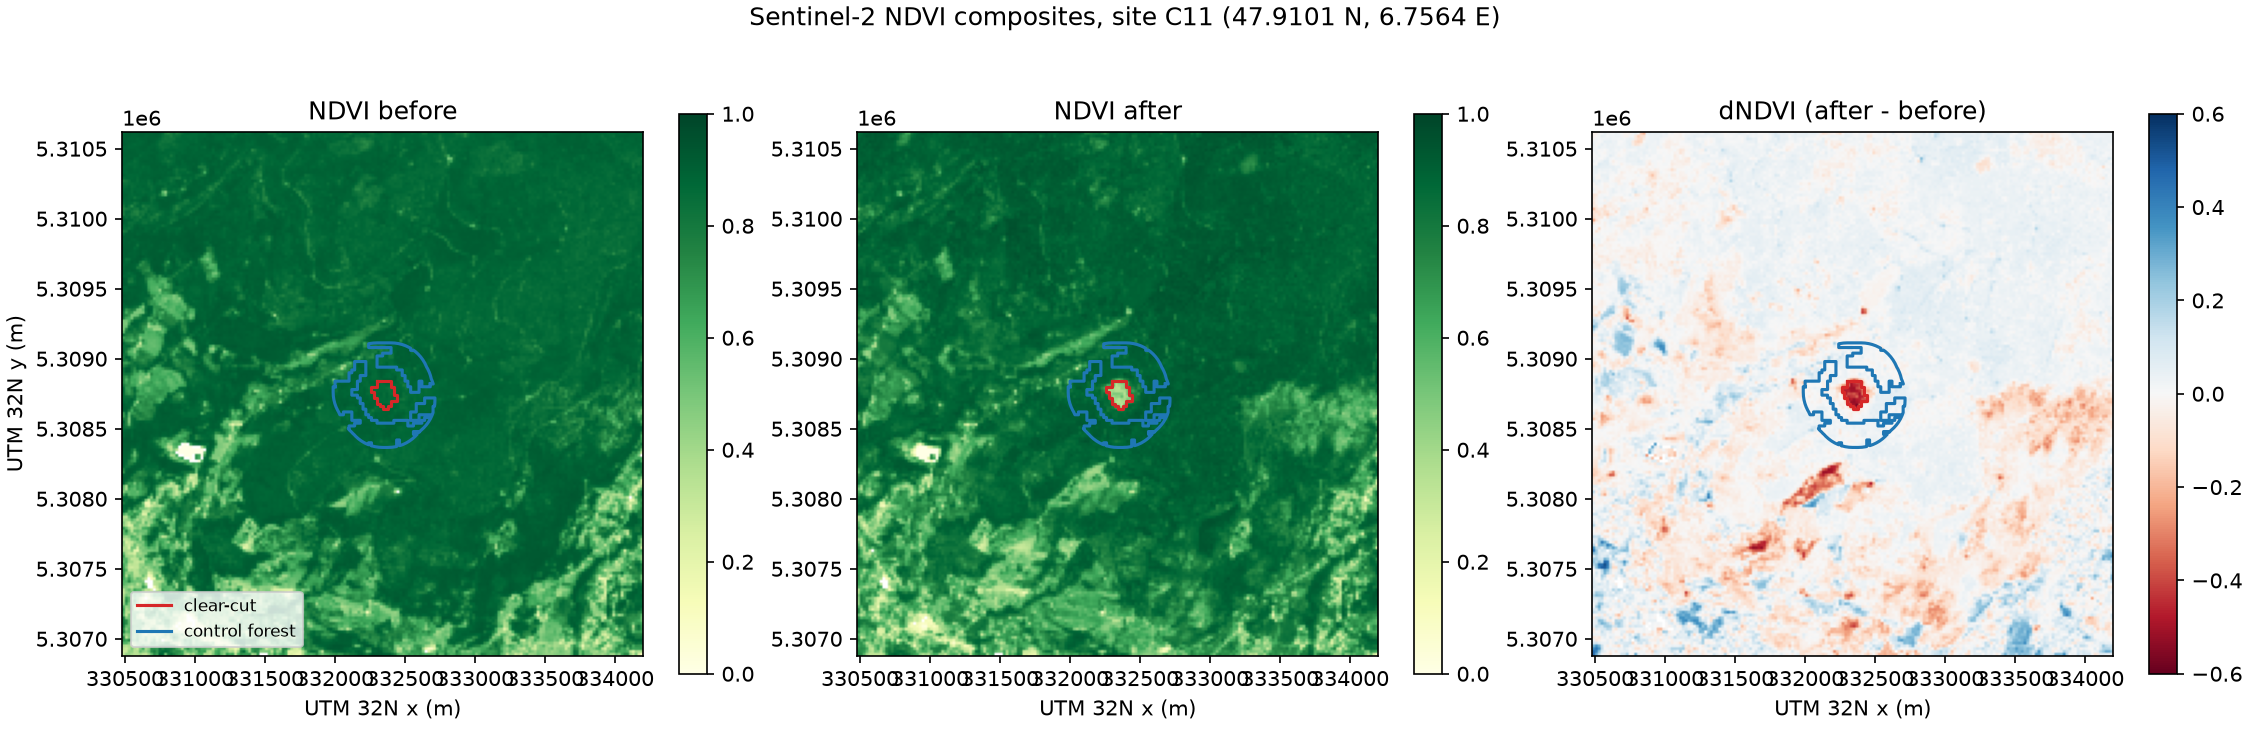
\includegraphics[width=\linewidth]{site_ndvi_maps.png}\\[0.3em]
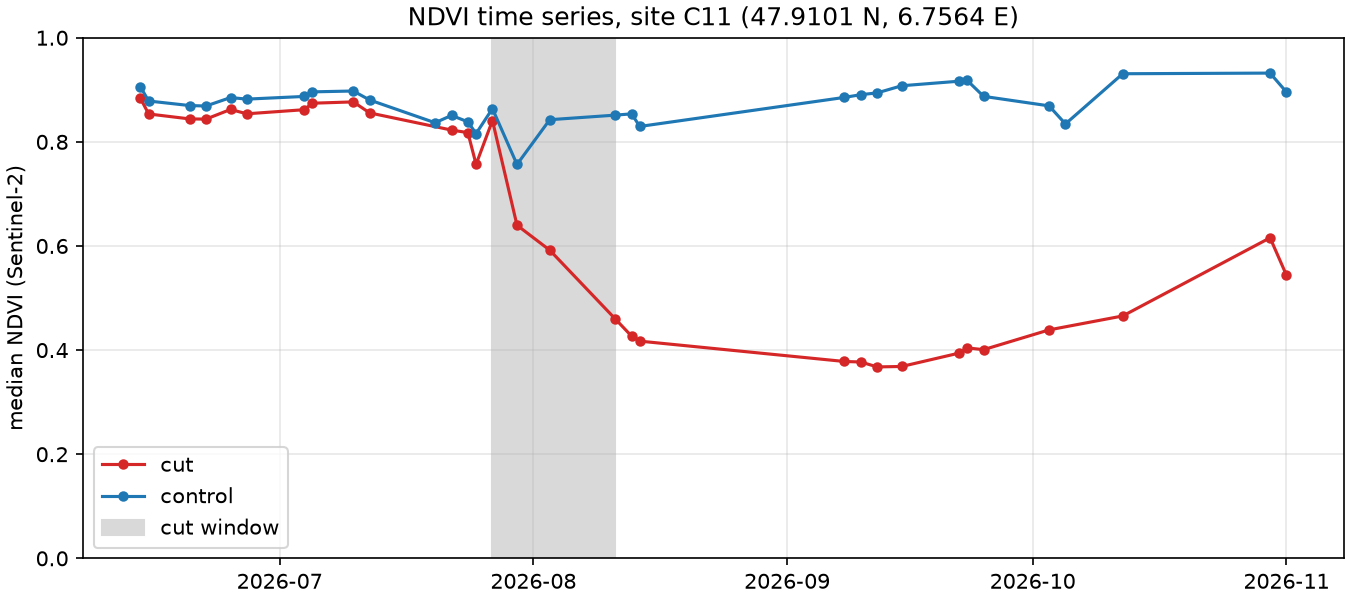
\includegraphics[width=0.85\linewidth]{site_ndvi_timeseries.png}
\caption{Site C11. Top: Sentinel-2 NDVI before (June--July), after (September--October) and difference, with the cut
(red) and the control forest (blue). Bottom: NDVI series of the cut and the control; the grey band is the cut
window.}
\label{fig-site}
\end{figure}

The NDVI of the cut drops from 0.84 (27/07) to 0.42--0.46 (11--13/08), while the control stays stable
(0.85--0.92).
\begin{itemize}
\item \textbf{Cut window}: we use the conservative window from 27/07 to 11/08.
\item \textbf{Control forest}: a ring of intact forest 100 to 275~m around the cut (548 pixels, 21.8~ha), sharing
  the slope, elevation and stand type of the cut. The 100~m margin avoids edge effects.
\end{itemize}

%=====================================================================
\section{Methods}

\subsection{Processing chain}

\paragraph{NISAR.} The L2 products are used as delivered by ISCE3:
\begin{itemize}
\item HH and HV $\gamma^0$ from GCOV, already terrain-corrected (RTC~\cite{small2011flattening});
\item HH coherence from GUNW: the \texttt{wrappedInterferogram} layer at 20~m and the
  \texttt{unwrappedInterferogram} layer at 80~m.
\end{itemize}
GUNW exists only in co-polarisation, so the HV information comes from GCOV only.

\paragraph{Sentinel-1.} Two SNAP~\cite{snap} graphs (\texttt{gpt}), versioned in the repository, are applied:
\begin{itemize}
\item \textbf{$\gamma^0$}: TOPSAR-Split, precise orbits, thermal noise removal, $\beta^0$ calibration, deburst,
  $4\times1$ multilook, Terrain-Flattening, then geocoding at 20~m (UTM 32N, Copernicus 30~m DEM).
\item \textbf{Coherence}: Back-Geocoding, then estimation over a $10\times3$ window after removing the flat-earth and
  topographic phases, deburst, then geocoding at 20~m. The ESD step is omitted because the site lies within a
  single burst (with no overlap, ESD returns zero coherence).
\end{itemize}

\paragraph{Common grid.} Every layer is resampled onto a 20~m UTM~32N grid covering the site plus 1.5~km:
\begin{itemize}
\item NISAR $\gamma^0$: average in linear power;
\item NISAR 20~m coherence: average;
\item Sentinel-1: bilinear interpolation.
\end{itemize}
$\gamma^0$ is then converted to dB.

\subsection{Change variables}

Each acquisition is classified relative to the cut window:
\begin{itemize}
\item \emph{before}: image, or coherence pair, entirely before 27/07;
\item \emph{after}: entirely after 11/08;
\item \emph{spanning}: pair bracketing the cut.
\end{itemize}
Before and after pairs are limited to 12--13~days. The spanning pair may reach 25~days, to include the 24-day NISAR
pair.

The variables, computed per sensor and per geometry, are:
\begin{itemize}
\item $\Delta\gamma^0$ = mean $\gamma^0$ after $-$ mean $\gamma^0$ before (dB), and $\gamma^0$ after;
\item coherence of the pair spanning the cut;
\item coherence drop = spanning pair $-$ coherence before;
\item $\Delta$ coherence = coherence after $-$ coherence before.
\end{itemize}

\subsection{Separability and detection measures}

For each variable, the cut pixels ($a$) are compared with the control pixels ($b$) using:
\begin{itemize}
\item the mean difference $\Delta=\bar a-\bar b$;
\item Cohen's d~\cite{cohen1988power};
\item the area under the ROC curve (AUC, Mann-Whitney statistic~\cite{hanley1982auc}), reported as
  $\max(\mathrm{AUC}, 1-\mathrm{AUC})$ (0.5: no separation; 1: perfect separation);
\item the Jeffries-Matusita distance~\cite{swain1978remote} (0 to 2).
\end{itemize}
Neighbouring pixels are spatially correlated, which would make p-values misleading. The 95~\% confidence intervals
of the AUC are therefore obtained by block bootstrap~\cite{kunsch1989bootstrap}: $3\times3$ pixel blocks (60~m;
$5\times5$ for 80~m layers), 300 draws.

\paragraph{Detection prototype.} Each variable is also evaluated as a detector over the whole window
($188\times187$ pixels, $3.7\times3.7$~km):
\begin{itemize}
\item \textbf{Reference}: Sentinel-2 dNDVI $\leq -0.3$ over forest (NDVI before $\geq 0.7$), with ambiguous
  partial changes excluded. This gives 95 cut pixels out of 25,723 (0.4~\%).
\item \textbf{Scores}: AUC over the window, F1 at the Otsu threshold~\cite{otsu1979threshold}, and maximum F1.
\end{itemize}

\paragraph{Checks.}
\begin{itemize}
\item Before the cut, cut and control must be indistinguishable.
\item A sensitivity analysis repeats the whole computation with polygons eroded by 20~m, which leaves 25
  \enquote{pure} cut pixels.
\end{itemize}

%=====================================================================
\section{Results}

\subsection{Check before the cut}

On acquisitions before the cut, the AUC between cut and control is 0.51 to 0.62 depending on the sensor and
variable. Both areas are radiometrically and interferometrically equivalent before the cut. This validates the
choice of the control: the differences measured afterwards can be attributed to the cut.

\subsection{Separability of the change variables}

\Cref{tab-core} compares the variables common to both sensors, and \cref{fig-auc} ranks all variables.
\Cref{tab-best} gives the best 20~m variable per sensor and geometry.

\begin{table}[htbp]
\centering
\scriptsize
\caption{Variables comparable across sensors (20 m): $\gamma^0$ change, coherence of the pair spanning the cut and coherence change (after $-$ before).}
\label{tab:core}
\begin{tabular}{llcrrlrrr}
\toprule
Sensor & Variable & $n_{bef}/n_{aft}$ & $\Delta$ & $d$ & AUC [95\,\% CI] & JM & win. AUC & F1$_{max}$ \\
\midrule
NISAR A144F26 & coherence of the pair over the cut HH & 2/6 & $-$0.40 & $-$3.9 & 1.00 [0.99--1.00] & 1.76 & 0.87 & 0.09 \\
NISAR A144F26 & $\Delta\gamma^0$ after $-$ before (dB) HV & 3/8 & $-$4.25 & $-$3.7 & 0.97 [0.93--0.99] & 1.28 & 0.84 & 0.27 \\
NISAR A144F26 & $\Delta\gamma^0$ after $-$ before (dB) HH & 3/8 & $-$4.22 & $-$3.2 & 0.96 [0.93--0.99] & 1.09 & 0.80 & 0.24 \\
NISAR A144F26 & $\Delta$ coherence after $-$ before HH & 2/6 & $-$0.08 & $-$1.1 & 0.77 [0.66--0.85] & 0.27 & 0.67 & 0.08 \\
\addlinespace
NISAR A72F26 & $\Delta\gamma^0$ after $-$ before (dB) HV & 3/7 & $-$3.72 & $-$3.0 & 0.94 [0.89--0.99] & 1.04 & 0.78 & 0.27 \\
NISAR A72F26 & $\Delta\gamma^0$ after $-$ before (dB) HH & 3/7 & $-$2.96 & $-$2.3 & 0.92 [0.86--0.97] & 0.82 & 0.78 & 0.22 \\
NISAR A72F26 & coherence of the pair over the cut HH & 3/5 & $-$0.25 & $-$1.8 & 0.91 [0.85--0.96] & 0.82 & 0.80 & 0.07 \\
NISAR A72F26 & $\Delta$ coherence after $-$ before HH & 3/5 & $-$0.05 & $-$0.7 & 0.65 [0.51--0.82] & 0.15 & 0.56 & 0.05 \\
\addlinespace
NISAR D138F64 & coherence of the pair over the cut HH & 1/5 & $-$0.31 & $-$3.7 & 1.00 [0.99--1.00] & 1.72 & 0.89 & 0.10 \\
NISAR D138F64 & $\Delta\gamma^0$ after $-$ before (dB) HV & 2/7 & $-$2.33 & $-$1.5 & 0.84 [0.78--0.89] & 0.44 & 0.71 & 0.14 \\
NISAR D138F64 & $\Delta\gamma^0$ after $-$ before (dB) HH & 2/7 & $-$1.69 & $-$1.1 & 0.72 [0.60--0.84] & 0.29 & 0.64 & 0.11 \\
NISAR D138F64 & $\Delta$ coherence after $-$ before HH & 1/5 & $-$0.01 & $-$0.1 & 0.55 [0.50--0.67] & 0.05 & 0.54 & 0.03 \\
\addlinespace
Sentinel-1 T139 & $\Delta\gamma^0$ after $-$ before (dB) VH & 4/8 & $-$2.20 & $-$2.1 & 0.91 [0.85--0.94] & 0.72 & 0.79 & 0.14 \\
Sentinel-1 T139 & $\Delta\gamma^0$ after $-$ before (dB) VV & 4/8 & $-$2.53 & $-$2.4 & 0.90 [0.82--0.95] & 0.76 & 0.87 & 0.22 \\
Sentinel-1 T139 & coherence of the pair over the cut VH & 3/7 & $-$0.06 & $-$0.8 & 0.74 [0.68--0.80] & 0.40 & 0.67 & 0.01 \\
Sentinel-1 T139 & coherence of the pair over the cut VV & 3/7 & $-$0.06 & $-$0.8 & 0.71 [0.60--0.80] & 0.17 & 0.63 & 0.04 \\
Sentinel-1 T139 & $\Delta$ coherence after $-$ before VV & 3/7 & 0.06 & 0.7 & 0.70 [0.59--0.78] & 0.13 & 0.66 & 0.02 \\
Sentinel-1 T139 & $\Delta$ coherence after $-$ before VH & 3/7 & 0.03 & 0.5 & 0.65 [0.55--0.73] & 0.11 & 0.61 & 0.01 \\
\bottomrule
\end{tabular}
\end{table}


\begin{figure}[p]
\centering
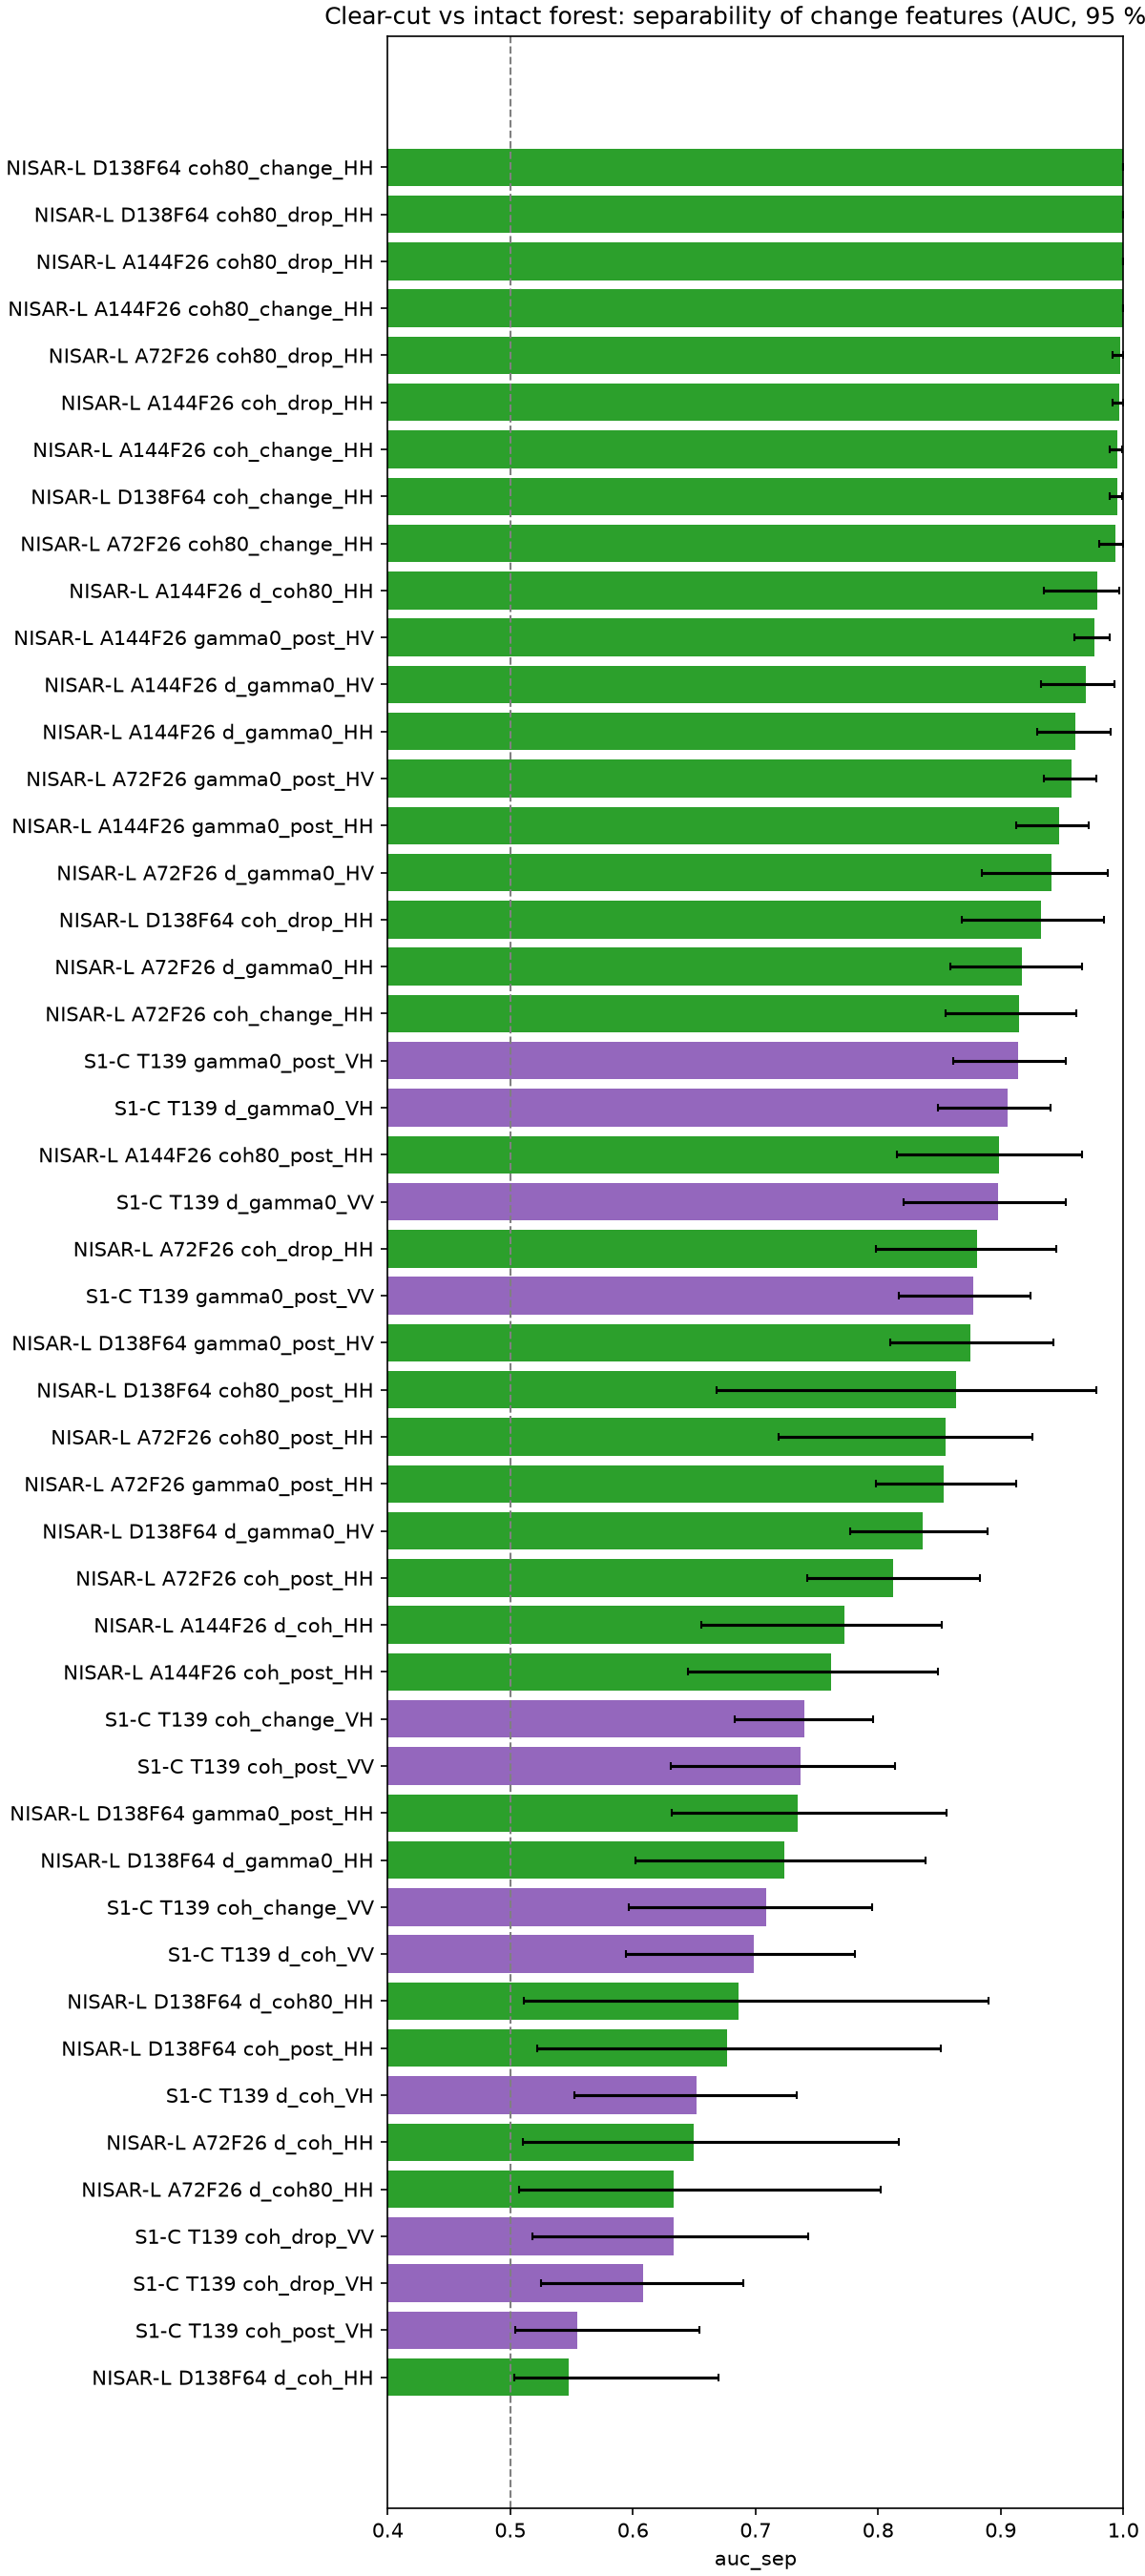
\includegraphics[height=0.92\textheight]{comparison_auc.png}
\caption{Cut / control separation AUC of all change variables, with 95~\% confidence intervals (block bootstrap).
Green: NISAR (L band); purple: Sentinel-1 (C band). The \texttt{coh80} variables are at 80~m and contain only about
4 independent pixels inside the cut.}
\label{fig-auc}
\end{figure}

\begin{table}[htbp]
\centering
\scriptsize
\caption{Best 20 m variable per sensor and geometry.}
\label{tab-best}
\begin{tabular}{llcrrlrrr}
\toprule
Sensor & Variable & $n_{bef}/n_{aft}$ & $\Delta$ & $d$ & AUC [95\,\% CI] & JM & win. AUC & F1$_{max}$ \\
\midrule
NISAR A144F26 & coherence drop (pair over the cut $-$ before) HH & 2/6 & $-$0.42 & $-$4.6 & 1.00 [0.99--1.00] & 1.82 & 0.82 & 0.29 \\
\addlinespace
NISAR D138F64 & coherence of the pair over the cut HH & 1/5 & $-$0.31 & $-$3.7 & 1.00 [0.99--1.00] & 1.72 & 0.89 & 0.10 \\
\addlinespace
NISAR A72F26 & $\gamma^0$ after (dB) HV & 3/7 & $-$3.56 & $-$2.3 & 0.96 [0.94--0.98] & 1.12 & 0.92 & 0.06 \\
\addlinespace
Sentinel-1 T139 & $\gamma^0$ after (dB) VH & 4/8 & $-$2.27 & $-$1.7 & 0.91 [0.86--0.95] & 0.67 & 0.86 & 0.04 \\
\bottomrule
\end{tabular}
\end{table}


\paragraph{Coherence.} This is the clearest difference between the two bands.
\begin{itemize}
\item \textbf{L band}: on the 24-day pair spanning the cut, NISAR coherence is 0.26--0.33 inside the cut against
  0.50--0.69 in the control forest. The AUC reaches 0.995 for A144 and D138, with a Cohen's d below $-3.7$.
\item \textbf{C band}: the forest is already decorrelated after 12~days (mean coherence 0.28). The Sentinel-1 pair
  spanning the cut separates it only weakly ($\Delta=-0.06$, AUC 0.71--0.74).
\item \textbf{After the cut}: the coherence difference between cut and forest becomes small again in both bands
  (AUC 0.55--0.77). Coherence therefore captures the cutting \emph{event}, not the final state.
\end{itemize}

\paragraph{Backscatter.} Both bands detect the cut; the L-band advantage depends on the geometry.
\begin{itemize}
\item \textbf{Cross-polarisation}: the drop reaches $-4.3$~dB for A144 (AUC 0.97) and $-3.7$~dB for A72
  (AUC 0.94), against $-2.2$~dB for Sentinel-1 VH (AUC 0.91).
\item \textbf{Co-polarisation}: $-4.2$~dB at HH (AUC 0.96) against $-2.5$~dB at VV (AUC 0.90).
\item \textbf{Geometry}: the descending NISAR geometry D138 is clearly less discriminating ($-2.3$~dB at HV,
  AUC 0.84).
\item \textbf{At equal geometry} (NISAR D138 and Sentinel-1 D139, both descending), the drop is similar ($-2.3$ vs
  $-2.2$~dB) and C band separates slightly better (AUC 0.91 vs 0.84). The L-band backscatter advantage therefore only
  appears in the ascending geometries.
\end{itemize}

\subsection{Time evolution and persistence of the contrast}

\Cref{fig-tsL,fig-tsC} show the time series of the cut and control, and \cref{fig-persist} the per-date
separation AUC.
\begin{itemize}
\item \textbf{L band}: HV $\gamma^0$ of the cut drops abruptly from $-9.2$ to $-13.7$~dB and stays at that level
  until November, while the control remains stable at $-9.2$~dB.
\item \textbf{C band}: the decrease is visible in August and September, then the cut returns to the forest level in
  October (VH AUC 0.52 on 25/10).
\end{itemize}
\Cref{tab-persistence} quantifies this behaviour. From August--September to October--November, the NISAR A144 HV AUC
only goes from 0.95 to 0.91, whereas the Sentinel-1 VV AUC drops from 0.86 to 0.66. In descending geometry,
however, the NISAR D138 HV AUC in October--November (0.76) is equivalent to the Sentinel-1 VH AUC (0.74): the better
L-band persistence is only established in ascending geometry.

\begin{figure}[htbp]
\centering
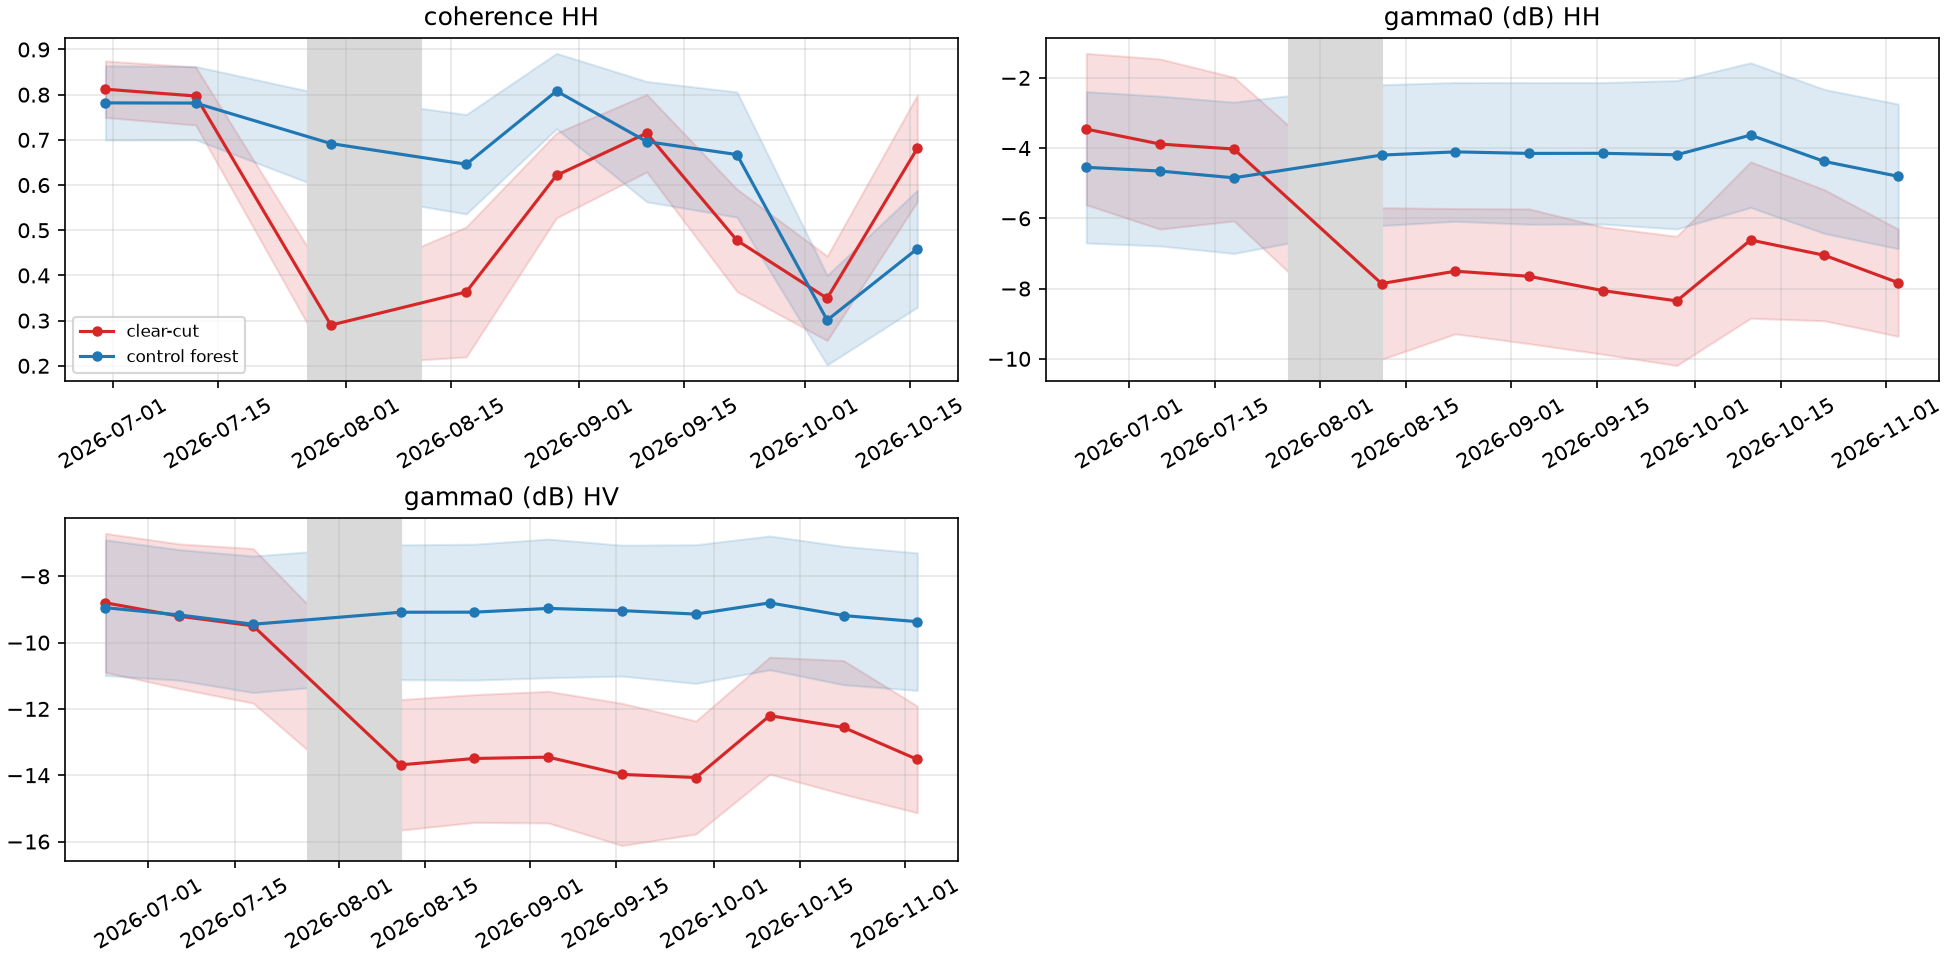
\includegraphics[width=\linewidth]{comparison_ts_NISAR-L_A144F26.png}
\caption{NISAR A144: HH coherence (pairs plotted at their mid-date), HH and HV $\gamma^0$ of the cut (red) and the
control (blue), mean $\pm$ standard deviation; the grey band is the cut window.}
\label{fig-tsL}
\end{figure}

\begin{figure}[htbp]
\centering
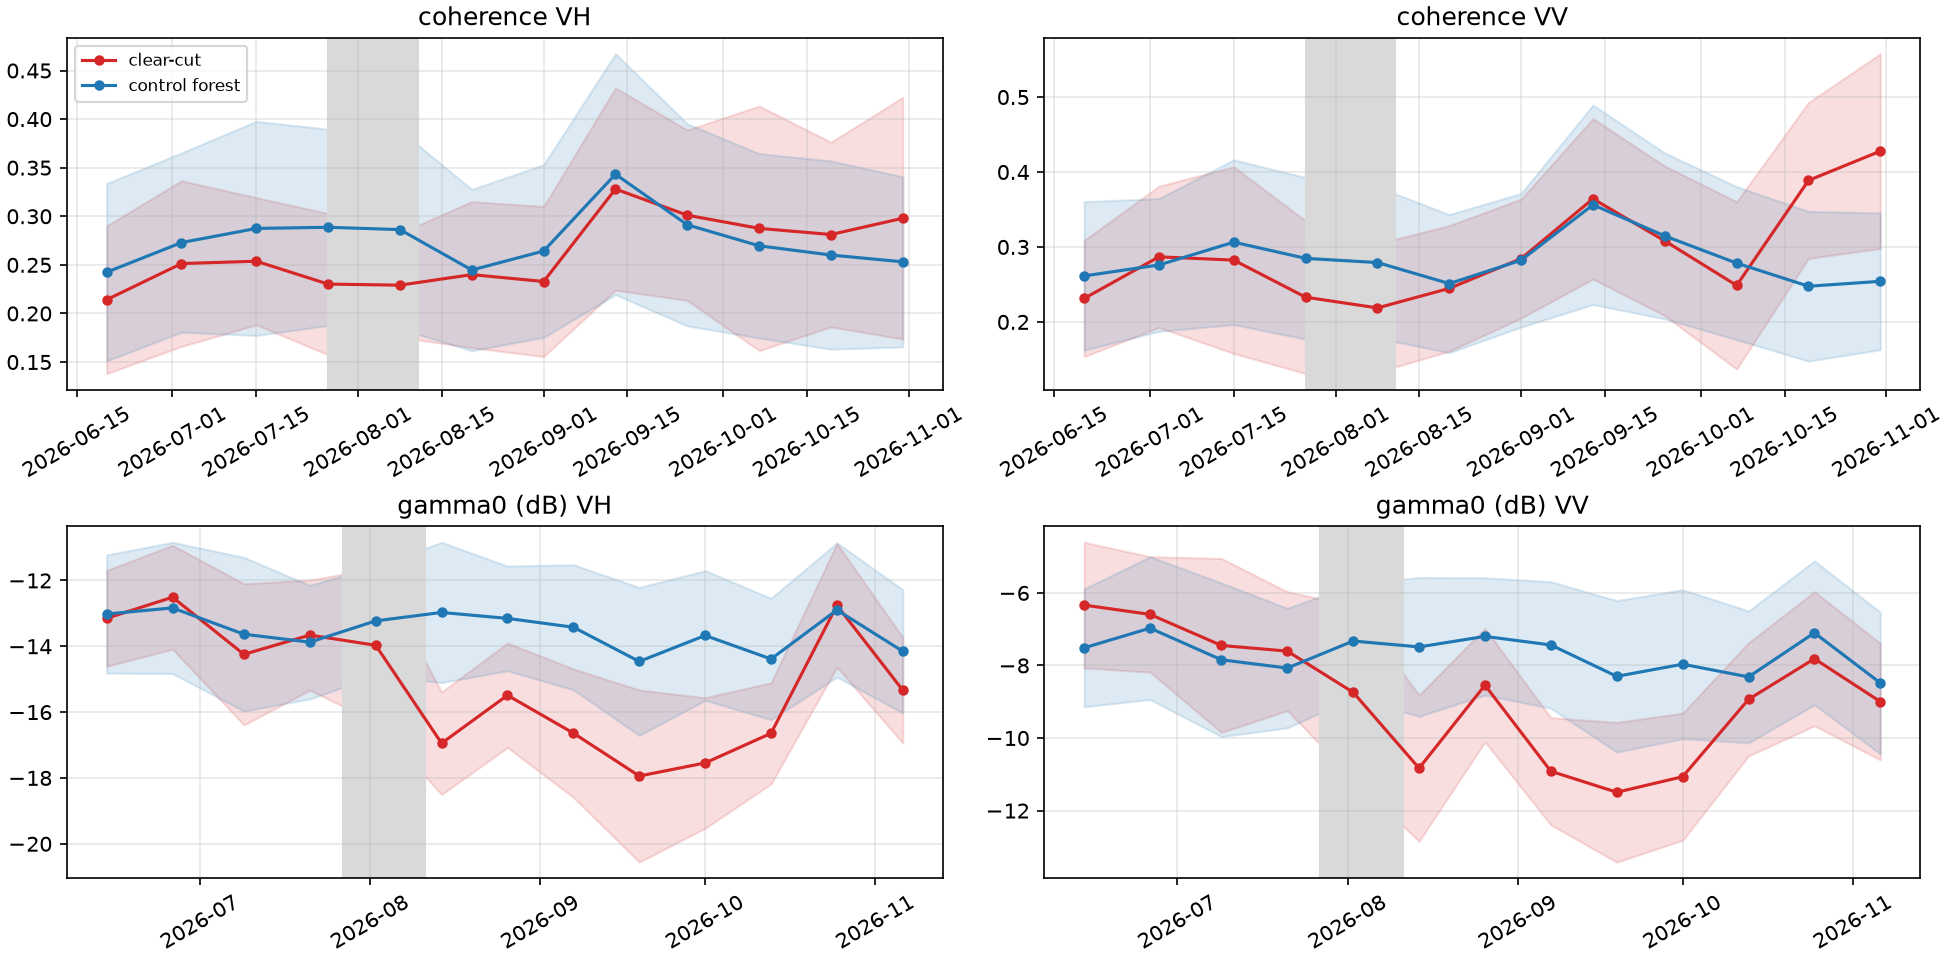
\includegraphics[width=\linewidth]{comparison_ts_S1-C_T139.png}
\caption{Sentinel-1 orbit 139: VH and VV coherence, VH and VV $\gamma^0$ of the cut (red) and the control (blue).}
\label{fig-tsC}
\end{figure}

\begin{figure}[htbp]
\centering
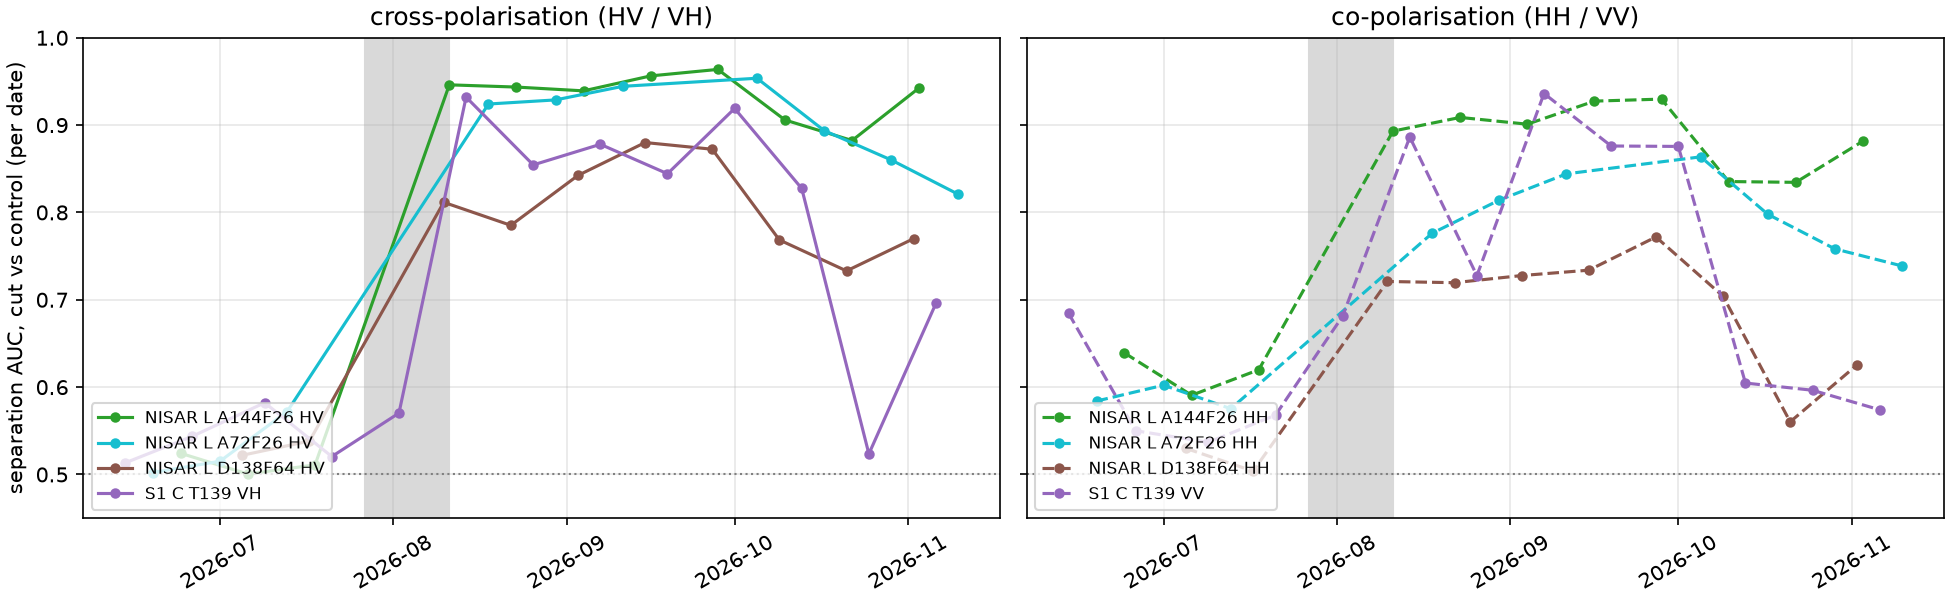
\includegraphics[width=\linewidth]{comparison_persistence.png}
\caption{Per-date cut / control separation AUC of backscatter, in cross-polarisation (left) and co-polarisation
(right). The contrast stays high at ascending L band and collapses in October at C band; in descending geometry, NISAR D138
and Sentinel-1 behave similarly.}
\label{fig-persist}
\end{figure}

\begin{table}[htbp]
\centering
\small
\caption{Persistence of the backscatter contrast after the cut: separation AUC and cut $-$ control difference, averaged per date over two periods.}
\label{tab-persistence}
\begin{tabular}{llrrrr}
\toprule
Sensor & Pol. & AUC Aug--Sep & $\Delta$ (dB) & AUC Oct--Nov & $\Delta$ (dB) \\
\midrule
NISAR A144F26 & HH & 0.91 & $-$3.7 & 0.85 & $-$2.9 \\
NISAR A144F26 & HV & 0.95 & $-$4.7 & 0.91 & $-$3.6 \\
NISAR A72F26 & HH & 0.81 & $-$2.6 & 0.79 & $-$2.3 \\
NISAR A72F26 & HV & 0.93 & $-$4.2 & 0.88 & $-$3.3 \\
NISAR D138F64 & HH & 0.74 & $-$2.0 & 0.63 & $-$1.0 \\
NISAR D138F64 & HV & 0.84 & $-$2.9 & 0.76 & $-$2.1 \\
Sentinel-1 T139 & VH & 0.88 & $-$3.3 & 0.74 & $-$1.8 \\
Sentinel-1 T139 & VV & 0.86 & $-$2.8 & 0.66 & $-$1.2 \\
\bottomrule
\end{tabular}
\end{table}


\subsection{Maps and detection prototype}

\Cref{fig-maps} shows the change maps around the site. The cut stands out clearly in NISAR HV $\Delta\gamma^0$ and
coherence, and in Sentinel-1 VH $\Delta\gamma^0$, but not in Sentinel-1 coherence.

Over the whole window, the detection AUC reaches 0.93 for NISAR HV $\gamma^0$ after the cut, and 0.86--0.87 for
Sentinel-1 $\gamma^0$. F1, however, stays low (maximum F1 of 0.29 at best). The cut represents only 0.4~\% of the
pixels, so a threshold on a single variable inevitably produces many false alarms.

\begin{figure}[htbp]
\centering
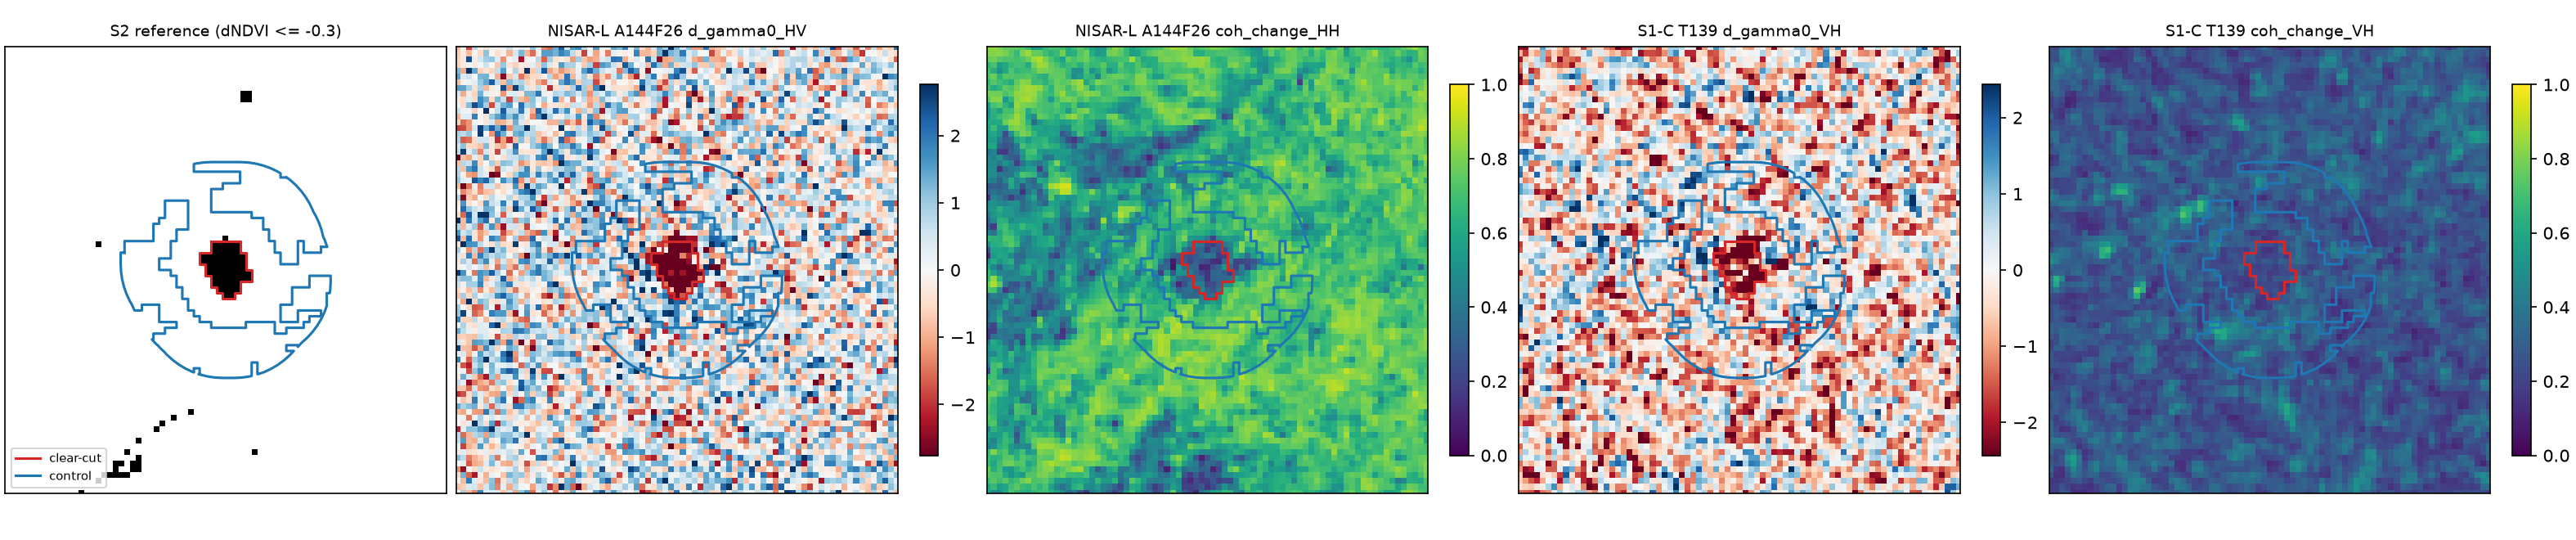
\includegraphics[width=\linewidth]{comparison_maps.png}
\caption{Maps around the site. From left to right: Sentinel-2 reference; NISAR A144 HV $\Delta\gamma^0$ and spanning
pair coherence; Sentinel-1 VH $\Delta\gamma^0$ and spanning pair coherence. Red: cut; blue: control.}
\label{fig-maps}
\end{figure}

\subsection{Sensitivity}

With polygons eroded by 20~m, every separability increases:
\begin{itemize}
\item A144 HV $\Delta\gamma^0$: AUC from 0.97 to 0.996;
\item A144 spanning pair coherence: from 0.995 to 0.999;
\item Sentinel-1 VH $\gamma^0$ after: from 0.91 to 0.98;
\item Sentinel-1 coherence: only from 0.74 to 0.80.
\end{itemize}
The conclusions therefore do not depend on edge pixels, and the L / C coherence gap remains.

\subsection{Synthesis at equal geometry}

\Cref{fig-summary} gathers the three key indicators for each geometry. The fairest comparison between bands is that
of the two descending geometries (NISAR D138 and Sentinel-1 D139, black outline).
\begin{itemize}
\item \textbf{Coherence}: L band wins in all three geometries (AUC 0.91--0.995 vs 0.74). This is the most robust
  result of the test.
\item \textbf{Backscatter and persistence}: L band wins in ascending geometry, but not at equal geometry, where both
  bands are on par (AUC 0.84 vs 0.91; persistence 0.76 vs 0.74).
\end{itemize}

\begin{figure}[htbp]
\centering
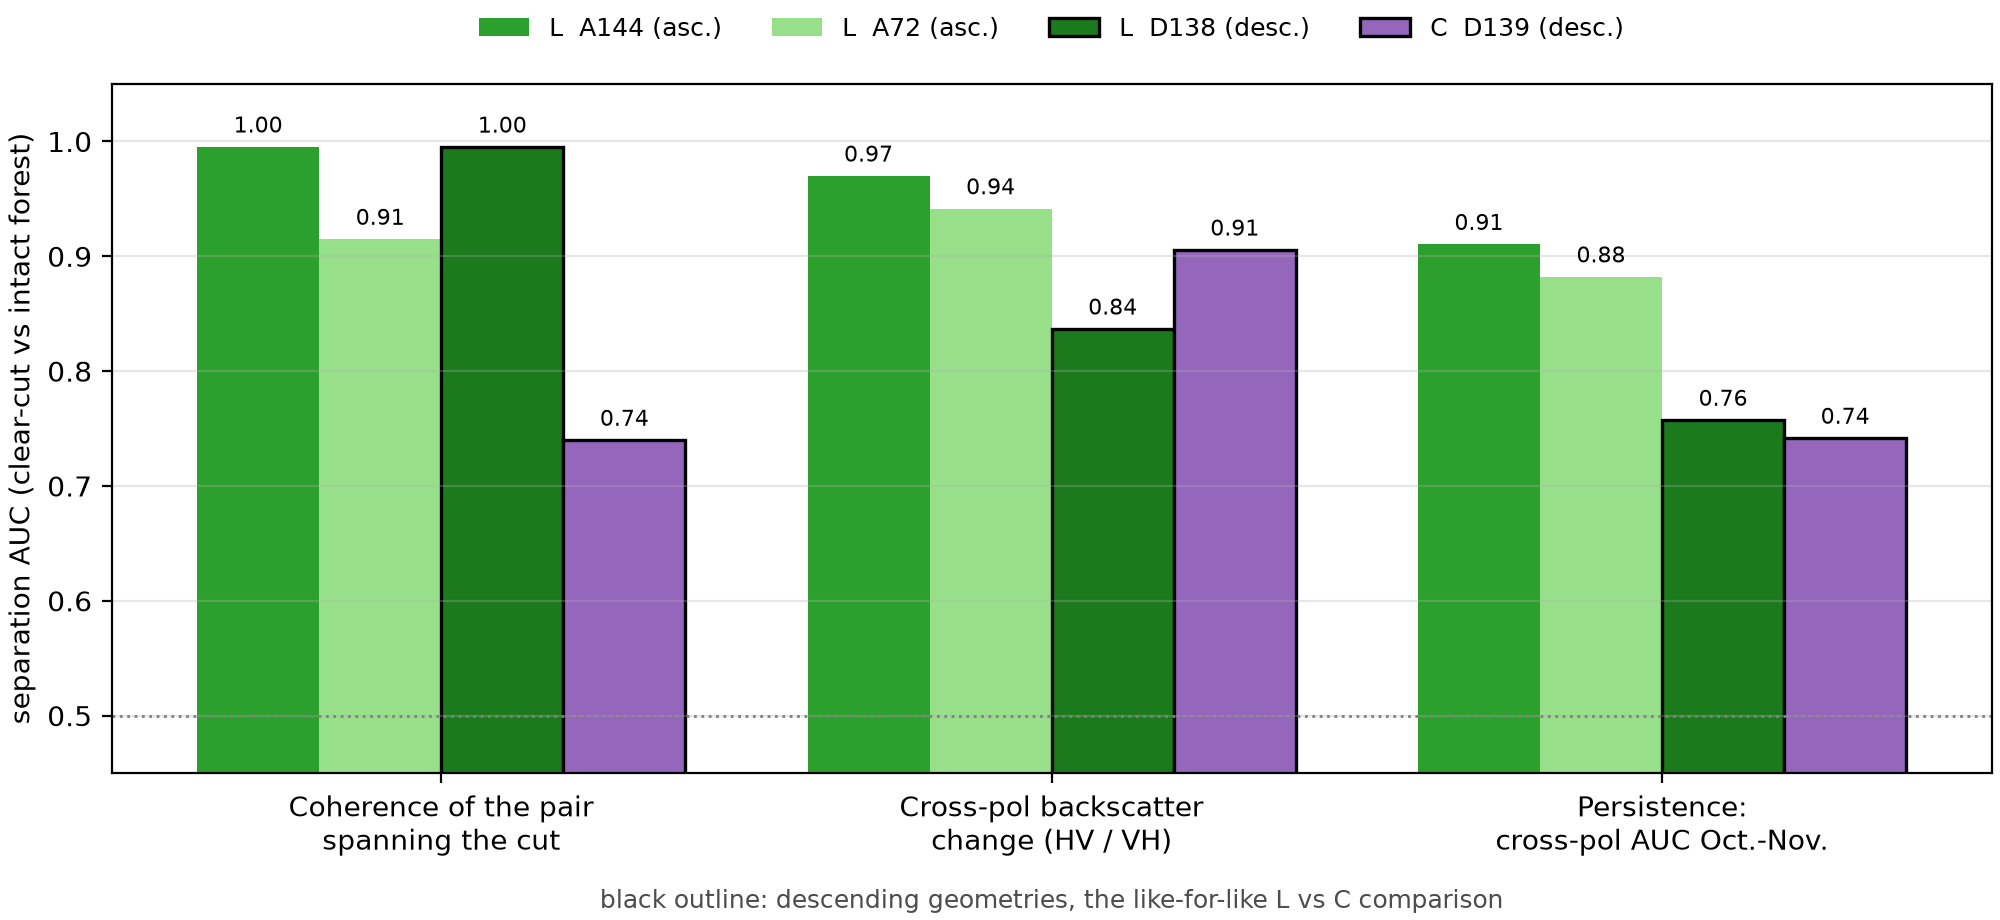
\includegraphics[width=0.9\linewidth]{summary_L_vs_C.png}
\caption{Cut / forest separation AUC for the three key indicators, per geometry (20~m grid). Black outline:
descending geometries, the like-for-like comparison between L and C band.}
\label{fig-summary}
\end{figure}

\subsection{Hypotheses assessment}

\begin{table}[htbp]
\centering\small
\caption{Assessment of the scoping hypotheses on site C11.}
\label{tab-hyp}
\begin{tabular}{lp{9.3cm}l}
\toprule
& Finding & Verdict \\
\midrule
H1 & 12-day forest coherence: 0.64--0.70 at L vs 0.28 at C. Even over 24~days, it is 0.69 at L. & confirmed \\
H2 & Coherence of the pair over the cut: AUC 0.995 at L vs 0.71--0.74 at C. & confirmed \\
H3 & Cross-pol $\Delta\gamma^0$: $-4.3$ and $-3.7$~dB (ascending L) vs $-2.2$~dB (C). At equal (descending)
geometry: $-2.3$~dB and AUC 0.84 at L vs 0.91 at C; similar persistence. & partial \\
H4 & At L band, HV $\geq$ HH in all three geometries (AUC 0.97 / 0.96, 0.94 / 0.92, 0.84 / 0.72). Coherence (HH)
does even better. & confirmed, nuanced \\
\bottomrule
\end{tabular}
\end{table}

%=====================================================================
\section{Discussion}

\paragraph{Physical interpretation.} The results agree with the wavelength.
\begin{itemize}
\item \textbf{L band} (24~cm) passes through the foliage and interacts with trunks and large branches. The forest
  therefore stays coherent over 12 to 24~days. Its HV backscatter, dominated by volume scattering, drops sharply
  when trees are felled and removed.
\item \textbf{C band} (5.6~cm) interacts mainly with leaves and twigs, which move with the wind. Temporal
  decorrelation is strong even without cutting~\cite{zebker1992decorrelation}, which explains the low value of C-band
  coherence for this purpose.
\item \textbf{Persistence}: C band is more sensitive to surface roughness and moisture. In autumn, the wet bare soil
  and logging residues of the cut scatter enough to match the forest. L band, less sensitive to these small
  structures, keeps the contrast. This behaviour is however only observed in ascending geometry, and the moisture
  explanation remains to be checked against weather data.
\end{itemize}
For operational monitoring this persistence is a major asset: a cut remains detectable at L band months after the
event, even if an acquisition is missed.

\paragraph{Dependence on conditions.} Coherence is strongly modulated by the weather.
\begin{itemize}
\item On the NISAR pair from 28/09 to 10/10, coherence falls to about 0.3 in the forest as well as in the cut,
  probably because of rain or wind.
\item A coherence-based detector must therefore compare each pair with a forest control from the same pair, as done
  here, rather than apply an absolute threshold.
\end{itemize}

\paragraph{Acquisition geometry.} The two ascending geometries (A144, A72) separate better than the descending one
(D138). In steep terrain, the edge and shadow effect of a cut depends on the look direction~\cite{bouvet2018shadow}.
The acquisition time also differs (around 6:20 local time in ascending, 20:40 in descending), which may change the
moisture and dew on the vegetation. These causes have not been disentangled. Two consequences:
\begin{itemize}
\item combining several geometries, which NISAR makes possible, is desirable;
\item a comparison between bands is only fair at equal geometry. Here it holds only for D138 vs Sentinel-1 D139, and
  it shows an L-band advantage for coherence only.
\end{itemize}

\paragraph{Complementarity of the two bands.} The Sentinel-1 revisit dates the cut more finely.
\begin{itemize}
\item On 02/08 no change is visible at C band (VH AUC 0.57); on 14/08 it is clear. Most of the cut therefore took
  place between 2 and 11~August, consistent with the NDVI.
\item The most robust system would combine C band for reactivity with L band for confirmation and persistence.
\end{itemize}

\paragraph{Limitations.}
\begin{enumerate}
\item \textbf{A single site} of 2.4~ha. Confidence intervals reflect pixel variability, not between-site variability.
  Replication on several cuts is needed (candidate C09 is available).
\item The NISAR pair over the cut is \textbf{24~days} long against 12 for Sentinel-1. This penalises L band, which
  strengthens the coherence conclusion. The estimators differ, however (number of looks), and the C-band coherence,
  close to zero, is limited by the estimator bias.
\item \textbf{A single Sentinel-1 orbit} (descending) against three NISAR geometries: the strict comparison between
  bands rests on a single geometry (D138).
\item The NISAR products are \textbf{provisional} (2026), and few pairs are available before the cut (1 to 3).
\item At 80~m the cut contains only about 4 independent pixels. The AUC values of 1 for the \texttt{coh80} layer are
  therefore indicative only.
\item The detection F1 is low, because of the very low prevalence and of thresholding a single variable.
  Operational detection would require:
  \begin{itemize}
  \item a combination of variables (HV $\gamma^0$ and coherence);
  \item spatial filtering (minimum object size);
  \item confirmation over several dates.
  \end{itemize}
\item Dieback (bark beetles) is frequent in the area. Its radar signature differs from that of a cut and was not
  studied here.
\end{enumerate}

%=====================================================================
\section{Reusable chain and perspectives}

\paragraph{A reusable chain.} The processing is organised as an importable Python package (\texttt{src/nisar\_s1});
the scripts only orchestrate it. The package covers:
\begin{itemize}
\item reading of ISCE3 NISAR L2 products, locally or remotely (\texttt{io\_nisar});
\item partial download (\texttt{download});
\item SNAP graphs and driver (\texttt{snap});
\item the common grid (\texttt{grid});
\item metrics (\texttt{stats}) and detection (\texttt{detect});
\item figures (\texttt{plots}).
\end{itemize}
Parameters are gathered in \texttt{config/params.yaml} and sites in GeoJSON: changing site amounts to providing a
new GeoJSON.

\paragraph{Towards ROSE-L.} The Copernicus ROSE-L mission (launch planned for 2028~\cite{esa2020rosel}) will provide
L-band data over Europe in continuity with NISAR. The chain developed here relies on standard quantities: RTC
$\gamma^0$, 12-day coherence and a common grid. It will be transferable by replacing the \texttt{io\_nisar} reader
with a reader for ROSE-L products. Since NISAR products are generated by the open-source ISCE3~\cite{isce3}, ISCE3
could also produce equivalent products from the level-1 data of both missions.

\paragraph{Proposed follow-up for the internship.}
\begin{itemize}
\item Replication on several cuts (including C09) and on dieback areas, to estimate between-site variability.
\item A multi-variable, multi-geometry detector (HV $\gamma^0$ and HH coherence) with temporal confirmation,
  validated on an independent reference.
\item Landslides under forest: comparison of NISAR and Sentinel-1 unwrapped interferograms. The high L-band coherence
  over forest shown here is precisely what C band lacks for interferometry under canopy.
\item P band (BIOMASS) on tropical sites, since it does not acquire over Europe.
\end{itemize}

%=====================================================================
\section{Conclusion}

On a 2.4~ha clear-cut in the Vosges, NISAR L band proves clearly more discriminating than Sentinel-1 C band in
coherence; for backscatter, its advantage depends on the geometry.
\begin{itemize}
\item \textbf{Coherence}: the pair spanning the cut separates cut and forest almost perfectly at L band
  (AUC 0.995), whereas C band adds almost nothing (AUC $\approx$ 0.72), the forest being already decorrelated.
\item \textbf{Backscatter}: in ascending geometry, the cross-polarisation drop is twice as strong at L band
  ($-4.3$ vs $-2.2$~dB). At equal (descending) geometry, C band performs as well (AUC 0.91 vs 0.84).
\item \textbf{Persistence}: in ascending geometry, the contrast persists at L band until November, whereas it weakens
  at C band in autumn; in descending geometry, both bands are on par.
\end{itemize}
These results confirm H1, H2 and H4, and partly H3: the decisive contribution of L band is interferometric. They
support the use of L band for forest-cut monitoring, which can be
continued with ROSE-L. They must be consolidated on more sites before designing an operational detector.

\printbibliography[heading=bibintoc,title={References}]

\appendix
%=====================================================================
\section{Reproduction}

The code is versioned; the data stay outside the repository, on an external disk. The conda environment is
\texttt{environment.yml}. Earthdata credentials are read from \texttt{.netrc}, which is never versioned.

\begin{verbatim}
python scripts/02_inventory.py               # ASF inventory
python scripts/03_site_candidates.py         # candidates (Sentinel-2)
python scripts/03b_verify_candidates.py      # temporal check
python scripts/03c_select_site.py --cand C11 # site and control forest
python scripts/04_fetch_nisar.py             # remote NISAR windows
python scripts/04_fetch_s1.py --start 2026-06-14 --end 2026-11-07
python scripts/05a_process_s1.py             # SNAP: 13 gamma0 and 12 coherences
python scripts/05b_compare.py                # comparison
python scripts/05b_compare.py --erode 20 --tag _erode20
python scripts/06_make_tables.py             # LaTeX tables FR and EN
\end{verbatim}

The tables of this report are generated automatically from the results
(\texttt{results/tables/comparison\_*.csv}); no number is copied by hand.

\section{Full separability table}

\begin{table}[htbp]
\centering
\scriptsize
\caption{Clear-cut / control forest separability of the change variables ($\Delta$: cut mean $-$ control mean; $d$: Cohen's d; AUC: max(AUC, 1$-$AUC) with block-bootstrap CI; JM: Jeffries-Matusita; win.\ AUC and F1$_{max}$: pixel-wise detection over the whole window, S2 dNDVI reference).}
\label{tab:separability}
\begin{tabular}{llcrrlrrr}
\toprule
Sensor & Variable & $n_{bef}/n_{aft}$ & $\Delta$ & $d$ & AUC [95\,\% CI] & JM & win. AUC & F1$_{max}$ \\
\midrule
NISAR A144F26 & coherence 80 m, pair over the cut HH & 2/6 & $-$0.43 & $-$6.0 & 1.00 [1.00--1.00] & 1.96 & 0.88 & 0.22 \\
NISAR A144F26 & coherence drop 80 m HH & 2/6 & $-$0.44 & $-$8.7 & 1.00 [1.00--1.00] & 1.98 & 0.86 & 0.33 \\
NISAR A144F26 & coherence drop (pair over the cut $-$ before) HH & 2/6 & $-$0.42 & $-$4.6 & 1.00 [0.99--1.00] & 1.82 & 0.82 & 0.29 \\
NISAR A144F26 & coherence of the pair over the cut HH & 2/6 & $-$0.40 & $-$3.9 & 1.00 [0.99--1.00] & 1.76 & 0.87 & 0.09 \\
NISAR A144F26 & $\Delta$ coherence 80 m HH & 2/6 & $-$0.08 & $-$2.3 & 0.98 [0.94--1.00] & 1.35 & 0.77 & 0.10 \\
NISAR A144F26 & $\gamma^0$ after (dB) HV & 3/8 & $-$4.22 & $-$2.6 & 0.98 [0.96--0.99] & 1.26 & 0.93 & 0.09 \\
NISAR A144F26 & $\Delta\gamma^0$ after $-$ before (dB) HV & 3/8 & $-$4.25 & $-$3.7 & 0.97 [0.93--0.99] & 1.28 & 0.84 & 0.27 \\
NISAR A144F26 & $\Delta\gamma^0$ after $-$ before (dB) HH & 3/8 & $-$4.22 & $-$3.2 & 0.96 [0.93--0.99] & 1.09 & 0.80 & 0.24 \\
NISAR A144F26 & $\gamma^0$ after (dB) HH & 3/8 & $-$3.34 & $-$2.1 & 0.95 [0.91--0.97] & 0.94 & 0.92 & 0.06 \\
NISAR A144F26 & coherence 80 m after HH & 2/6 & $-$0.06 & $-$1.4 & 0.90 [0.81--0.97] & 1.19 & 0.83 & 0.03 \\
NISAR A144F26 & $\Delta$ coherence after $-$ before HH & 2/6 & $-$0.08 & $-$1.1 & 0.77 [0.66--0.85] & 0.27 & 0.67 & 0.08 \\
NISAR A144F26 & coherence after HH & 2/6 & $-$0.06 & $-$0.9 & 0.76 [0.65--0.85] & 0.30 & 0.76 & 0.02 \\
\addlinespace
NISAR A72F26 & coherence drop 80 m HH & 3/5 & $-$0.24 & $-$3.6 & 1.00 [0.99--1.00] & 1.64 & 0.76 & 0.29 \\
NISAR A72F26 & coherence 80 m, pair over the cut HH & 3/5 & $-$0.27 & $-$3.3 & 0.99 [0.98--1.00] & 1.74 & 0.83 & 0.24 \\
NISAR A72F26 & $\gamma^0$ after (dB) HV & 3/7 & $-$3.56 & $-$2.3 & 0.96 [0.94--0.98] & 1.12 & 0.92 & 0.06 \\
NISAR A72F26 & $\Delta\gamma^0$ after $-$ before (dB) HV & 3/7 & $-$3.72 & $-$3.0 & 0.94 [0.89--0.99] & 1.04 & 0.78 & 0.27 \\
NISAR A72F26 & $\Delta\gamma^0$ after $-$ before (dB) HH & 3/7 & $-$2.96 & $-$2.3 & 0.92 [0.86--0.97] & 0.82 & 0.78 & 0.22 \\
NISAR A72F26 & coherence of the pair over the cut HH & 3/5 & $-$0.25 & $-$1.8 & 0.91 [0.85--0.96] & 0.82 & 0.80 & 0.07 \\
NISAR A72F26 & coherence drop (pair over the cut $-$ before) HH & 3/5 & $-$0.22 & $-$1.8 & 0.88 [0.80--0.94] & 0.62 & 0.74 & 0.13 \\
NISAR A72F26 & coherence 80 m after HH & 3/5 & $-$0.05 & $-$1.3 & 0.86 [0.72--0.93] & 0.57 & 0.71 & 0.02 \\
NISAR A72F26 & $\gamma^0$ after (dB) HH & 3/7 & $-$2.35 & $-$1.5 & 0.85 [0.80--0.91] & 0.47 & 0.85 & 0.04 \\
NISAR A72F26 & coherence after HH & 3/5 & $-$0.08 & $-$1.2 & 0.81 [0.74--0.88] & 0.36 & 0.71 & 0.02 \\
NISAR A72F26 & $\Delta$ coherence after $-$ before HH & 3/5 & $-$0.05 & $-$0.7 & 0.65 [0.51--0.82] & 0.15 & 0.56 & 0.05 \\
NISAR A72F26 & $\Delta$ coherence 80 m HH & 3/5 & $-$0.02 & $-$0.5 & 0.63 [0.51--0.80] & 0.06 & 0.54 & 0.01 \\
\addlinespace
NISAR D138F64 & coherence drop 80 m HH & 1/5 & $-$0.28 & $-$4.7 & 1.00 [1.00--1.00] & 1.86 & 0.86 & 0.34 \\
NISAR D138F64 & coherence 80 m, pair over the cut HH & 1/5 & $-$0.28 & $-$6.8 & 1.00 [1.00--1.00] & 2.00 & 0.87 & 0.08 \\
NISAR D138F64 & coherence of the pair over the cut HH & 1/5 & $-$0.31 & $-$3.7 & 1.00 [0.99--1.00] & 1.72 & 0.89 & 0.10 \\
NISAR D138F64 & coherence drop (pair over the cut $-$ before) HH & 1/5 & $-$0.28 & $-$2.4 & 0.93 [0.87--0.98] & 0.92 & 0.81 & 0.24 \\
NISAR D138F64 & $\gamma^0$ after (dB) HV & 2/7 & $-$2.52 & $-$1.5 & 0.88 [0.81--0.94] & 0.55 & 0.86 & 0.05 \\
NISAR D138F64 & coherence 80 m after HH & 1/5 & $-$0.04 & $-$2.0 & 0.86 [0.67--0.98] & 0.63 & 0.60 & 0.01 \\
NISAR D138F64 & $\Delta\gamma^0$ after $-$ before (dB) HV & 2/7 & $-$2.33 & $-$1.5 & 0.84 [0.78--0.89] & 0.44 & 0.71 & 0.14 \\
NISAR D138F64 & $\gamma^0$ after (dB) HH & 2/7 & $-$1.47 & $-$0.8 & 0.73 [0.63--0.86] & 0.16 & 0.75 & 0.04 \\
NISAR D138F64 & $\Delta\gamma^0$ after $-$ before (dB) HH & 2/7 & $-$1.69 & $-$1.1 & 0.72 [0.60--0.84] & 0.29 & 0.64 & 0.11 \\
NISAR D138F64 & $\Delta$ coherence 80 m HH & 1/5 & $-$0.04 & $-$0.7 & 0.69 [0.51--0.89] & 0.12 & 0.63 & 0.02 \\
NISAR D138F64 & coherence after HH & 1/5 & $-$0.03 & $-$0.7 & 0.68 [0.52--0.85] & 0.13 & 0.62 & 0.02 \\
NISAR D138F64 & $\Delta$ coherence after $-$ before HH & 1/5 & $-$0.01 & $-$0.1 & 0.55 [0.50--0.67] & 0.05 & 0.54 & 0.03 \\
\addlinespace
Sentinel-1 T139 & $\gamma^0$ after (dB) VH & 4/8 & $-$2.27 & $-$1.7 & 0.91 [0.86--0.95] & 0.67 & 0.86 & 0.04 \\
Sentinel-1 T139 & $\Delta\gamma^0$ after $-$ before (dB) VH & 4/8 & $-$2.20 & $-$2.1 & 0.91 [0.85--0.94] & 0.72 & 0.79 & 0.14 \\
Sentinel-1 T139 & $\Delta\gamma^0$ after $-$ before (dB) VV & 4/8 & $-$2.53 & $-$2.4 & 0.90 [0.82--0.95] & 0.76 & 0.87 & 0.22 \\
Sentinel-1 T139 & $\gamma^0$ after (dB) VV & 4/8 & $-$1.92 & $-$1.5 & 0.88 [0.82--0.92] & 0.51 & 0.86 & 0.04 \\
Sentinel-1 T139 & coherence of the pair over the cut VH & 3/7 & $-$0.06 & $-$0.8 & 0.74 [0.68--0.80] & 0.40 & 0.67 & 0.01 \\
Sentinel-1 T139 & coherence after VV & 3/7 & 0.04 & 0.9 & 0.74 [0.63--0.81] & 0.18 & 0.68 & 0.02 \\
Sentinel-1 T139 & coherence of the pair over the cut VV & 3/7 & $-$0.06 & $-$0.8 & 0.71 [0.60--0.80] & 0.17 & 0.63 & 0.04 \\
Sentinel-1 T139 & $\Delta$ coherence after $-$ before VV & 3/7 & 0.06 & 0.7 & 0.70 [0.59--0.78] & 0.13 & 0.66 & 0.02 \\
Sentinel-1 T139 & $\Delta$ coherence after $-$ before VH & 3/7 & 0.03 & 0.5 & 0.65 [0.55--0.73] & 0.11 & 0.61 & 0.01 \\
Sentinel-1 T139 & coherence drop (pair over the cut $-$ before) VV & 3/7 & $-$0.04 & $-$0.4 & 0.63 [0.52--0.74] & 0.08 & 0.57 & 0.01 \\
Sentinel-1 T139 & coherence drop (pair over the cut $-$ before) VH & 3/7 & $-$0.03 & $-$0.3 & 0.61 [0.53--0.69] & 0.15 & 0.59 & 0.01 \\
Sentinel-1 T139 & coherence after VH & 3/7 & 0.01 & 0.2 & 0.55 [0.50--0.65] & 0.02 & 0.57 & 0.01 \\
\bottomrule
\end{tabular}
\end{table}


\end{document}
